\chapter{Theorem registry and proof dependencies}\label{app:crosswalk}

The source registry contains 128 records across the coordinated volumes; 68 are assigned to this volume. The crosswalk below identifies them by their original registry IDs (the prefix \texttt{F.} is omitted; for example \texttt{T51} stands for \texttt{F.T51}). It lists the statement kind recorded in the registry, the registered scope tag, the registry chapter (the order in which a result was first released) and the location in this manuscript. The two chapter schemes differ for a few records, because results are placed here where they are first needed: \texttt{T31} (monotone orbits) is in Chapter~\ref{ch:growth}, and \texttt{T44}, \texttt{T47} (the \(\gamma\)-framework and the bounded window) are in Chapter~\ref{ch:persist}. Registered corrections and open problems are included, so that every record can be traced.

\footnotesize
\begin{longtable}{@{}p{13mm}p{45mm}p{33mm}p{8mm}p{12mm}p{17mm}@{}}
\toprule ID & Source record title & Source status & Scope & Reg.\ chap. & Here\\\midrule\endfirsthead
\toprule ID & Source record title & Source status & Scope & Reg.\ chap. & Here\\\midrule\endhead
\texttt{CDEF} & G1-C collective map C & PROPOSED & C & II.1 & Def.~\ref{th:F.CDEF} \\
\texttt{T17p} & Delta\_coll is reduced & PROVED+CHECKED & A0 & II.1 & Prop.~\ref{th:F.T17p} \\
\texttt{T17} & Plateau law & PROVED+CHECKED & C & II.1 & Prop.~\ref{th:F.T17} \\
\texttt{T18} & Growth-time bound & PROVED+CHECKED & C & II.1 & Thm~\ref{th:F.T18} \\
\texttt{T19} & Collective fibre growth & PROVED & C & II.1 & Thm~\ref{th:F.T19} \\
\texttt{T26} & Exact global minimum of the growth-time bound & PROVED+CHECKED & C & II.1 & Prop.~\ref{th:F.T26} \\
\texttt{T27} & Provable lower bound for growth of R & PROVED+CHECKED & C & II.1 & Prop.~\ref{th:F.T27} \\
\texttt{T28} & Monotone fibre growth is specific to the collective branch & PROVED+CHECKED & C & II.1 & Ex.~\ref{th:F.T28} \\
\texttt{T30} & Arithmetic of G & PROVED & A0 & II.2 & Thm~\ref{th:F.T30} \\
\texttt{T31} & Monotone orbits & PROVED & C & II.2 & Thm~\ref{th:F.T31} \\
\texttt{T32} & Regime I: closed dynamics for G=1 & PROVED & C & II.2 & Thm~\ref{th:F.T32} \\
\texttt{T33} & Non-universality of reach & CORRECTED & C & II.2 & Thm~\ref{th:F.T33} \\
\texttt{T34} & G=2 cannot persist & PROVED & C & II.2 & Thm~\ref{th:F.T34} \\
\texttt{L1} & Modular escape from any fixed fibre & PROVED & C & II.2 & Lem.~\ref{th:F.L1} \\
\texttt{L2} & Universal collapse for G=2,3,6 & PROVED & C & II.2 & Thm~\ref{th:F.L2} \\
\texttt{L3} & Exact eventual three-step scaling in regime I & PROVED & C & II.2 & Thm~\ref{th:F.L3} \\
\texttt{L4} & Exact reach counting for G=1 & PROVED & C & II.2 & Thm~\ref{th:F.L4} \\
\texttt{L5} & Scope erratum to v005 T33 & CORRECTED & C & II.2 & Rem.~\ref{th:F.L5} \\
\texttt{L6} & Full collapse to G=1 (problem) & FALSE & C & II.3 & Rem.~\ref{th:F.L6} \\
\texttt{T35} & Transition criterion & PROVED & C & II.3 & Thm~\ref{th:F.T35} \\
\texttt{T36} & Anatomy of a preserving event & PROVED & C & II.3 & Thm~\ref{th:F.T36} \\
\texttt{T37} & Plateau escape & PROVED & C & II.3 & Prop.~\ref{th:F.T37} \\
\texttt{T38} & Persistent regime P\_g (counterexample to collapse) & PROVED+CHECKED & C & II.3 & Thm~\ref{th:F.T38} \\
\texttt{T38a} & Existence of P\_g for every such g & PROVED+CHECKED & C & II.3 & Prop.~\ref{th:F.T38a} \\
\texttt{T39} & Universal G-collapse is false & PROVED+CHECKED & C & II.3 & Thm~\ref{th:F.T39} \\
\texttt{T40} & Reach set and growth in P\_g & PROVED & C & II.3 & Thm~\ref{th:F.T40} \\
\texttt{T41} & Status of other g (problem) & CORRECTED & C & II.3 & Rem.~\ref{th:F.T41} \\
\texttt{T42} & Elementary construction of P\_g & PROVED+CHECKED & C & II.3 & Thm~\ref{th:F.T42} \\
\texttt{T43} & Periodic increment of fibre size & PROVED+CHECKED & C & II.3 & Thm~\ref{th:F.T43} \\
\texttt{T44} & The gamma-framework & PROVED+CHECKED & C & II.4 & Thm~\ref{th:F.T44} \\
\texttt{T45} & G\_inf cannot divide 24 & PROVED+CHECKED & C & II.3 & Thm~\ref{th:F.T45} \\
\texttt{T46} & Persistent regimes with gcd(g,6)>1 (Theorem P*) & PROVED+CHECKED & C & II.3 & Thm~\ref{th:F.T46} \\
\texttt{T47} & Persistent orbits live in a bounded gamma-window & PROVED & C & II.4 & Thm~\ref{th:F.T47} \\
\texttt{T48} & Scaling question (M4a, M4b) & FALSE & C & II.4 & Rem.~\ref{th:F.T48} \\
\texttt{T49} & The one-step law & PROVED+CHECKED & C & II.4 & Thm~\ref{th:F.T49} \\
\texttt{T50} & The eight-step theorem (G=11) & PROVED+CHECKED & C & II.4 & Thm~\ref{th:F.T50} \\
\texttt{T51} & Finite-state closure: every persistent orbit scales exactly & PROVED & C & II.4 & Thm~\ref{th:F.T51} \\
\texttt{T52} & The window theorem & PROVED & C & II.4 & Thm~\ref{th:F.T52} \\
\texttt{T53} & The absorption criterion & PROVED & C & II.4 & Thm~\ref{th:F.T53} \\
\texttt{T54} & Carry completeness & PROVED & C & II.4 & Thm~\ref{th:F.T54} \\
\texttt{T55} & Eventual carries are prime powers & PROVED & C & II.4 & Thm~\ref{th:F.T55} \\
\texttt{T56} & The decoupled odometer law & PROVED+CHECKED & C & II.4 & Thm~\ref{th:F.T56} \\
\texttt{T57} & General q-carry theorem & PROVED+CHECKED & C & II.4 & Thm~\ref{th:F.T57} \\
\texttt{T58} & Corrections to v008 & CORRECTED & C & II.4 & Rem.~\ref{th:F.T58} \\
\texttt{T59} & The carry scheduler & PROVED+CHECKED & C & II.5 & Thm~\ref{th:F.T59} \\
\texttt{T60} & Single-prime dominance & PROVED+CHECKED & C & II.5 & Thm~\ref{th:F.T60} \\
\texttt{T61} & The eventual scaling factor is a prime power & PROVED+CHECKED & C & II.5 & Thm~\ref{th:F.T61} \\
\texttt{T62} & Two saturated clocks have coprime periods & PROVED+CHECKED & C & II.5 & Thm~\ref{th:F.T62} \\
\texttt{T63} & Corrections to the v010 problem statement & CORRECTED & C & II.5 & Rem.~\ref{th:F.T63} \\
\texttt{T67} & Exact carry-level predictor & PROVED+CHECKED & C & II.6 & Thm~\ref{th:F.T67} \\
\texttt{T64} & Minimax selection theorem & PROVED+CHECKED & C & II.6 & Thm~\ref{th:F.T64} \\
\texttt{T65} & Quotient-residue formula & PROVED+CHECKED & C & II.6 & Thm~\ref{th:F.T65} \\
\texttt{T66} & Static survivor certificate & PROVED+CHECKED & C & II.6 & Thm~\ref{th:F.T66} \\
\texttt{T68} & Consequences of static certification & CORRECTED & C & II.6 & Thm~\ref{th:F.T68} \\
\texttt{T69} & Reset-descent bound (sharp) & PROVED+CHECKED & C & II.7 & Thm~\ref{th:F.T69} \\
\texttt{T70} & Class-counting entry bound & PROVED+CHECKED & C & II.7 & Thm~\ref{th:F.T70} \\
\texttt{T71} & Polynomial entry bound & PROVED+CHECKED & C & II.7 & Thm~\ref{th:F.T71} \\
\texttt{T72} & Dynamic-G effective bound & PROVED+CHECKED & C & II.7 & Thm~\ref{th:F.T72} \\
\texttt{T73} & Registered corrections and scope (v012) & CORRECTED & C & II.7 & Thm~\ref{th:F.T73} \\
\texttt{O12.1} & Exact transient time / near-sharp bound & OPEN & C & II.7 & Prob.~\ref{th:O12.1} \\
\texttt{O12.2} & Static certificate for composite/even g & OPEN & C & II.7 & Prob.~\ref{th:O12.2} \\
\texttt{O12.3} & T71 where T67 does not apply & OPEN & C & II.7 & Prob.~\ref{th:O12.3} \\
\texttt{O12.4} & Closed-form m\_p and survivor for q-carry families & OPEN & C & II.6 & Prob.~\ref{th:O12.4} \\
\texttt{O12.5} & Infinitely many carry sizes & OPEN & C & II.4 & Prob.~\ref{th:O12.5} \\
\texttt{O12.6} & q=11 class-closure certificate (g=6689) & OPEN & C & II.4 & Prob.~\ref{th:O12.6} \\
\texttt{O10.3} & Realisable triples (g, p, Abs\_p) & OPEN & C & II.5 & Prob.~\ref{th:O10.3} \\
\texttt{O10.4} & Composite/even g sample & OPEN & C & II.5 & Prob.~\ref{th:O10.4} \\
\texttt{E71} & Post-freeze numerical erratum to the T71 data sentence & CORRECTED & C & II.7 & Rem.~\ref{th:F.E71} \\
\bottomrule
\end{longtable}
\normalsize


\section*{Proof dependencies}

The table at the end of this appendix gives the registry's direct dependency list for each record, and Figure~\ref{fig:dag} draws the same relations by manuscript chapter, with the main line of the argument highlighted: from the fibre theorem (\texttt{T1}) and the collective rule (\texttt{CDEF}) through monotonicity (\texttt{T31}), the \(\gamma\)-framework (\texttt{T44}), the one-step law (\texttt{T49}), class closure (\texttt{T51}), carry completeness and prime-power carries (\texttt{T54}, \texttt{T55}), the odometer law (\texttt{T56}), single-prime dominance (\texttt{T60}), minimax selection and the exact predictor (\texttt{T64}, \texttt{T67}), the static certificate (\texttt{T66}), and the entry and dynamic-\(G\) bounds (\texttt{T70}, \texttt{T72}).

\begin{figure}[t]
\centering
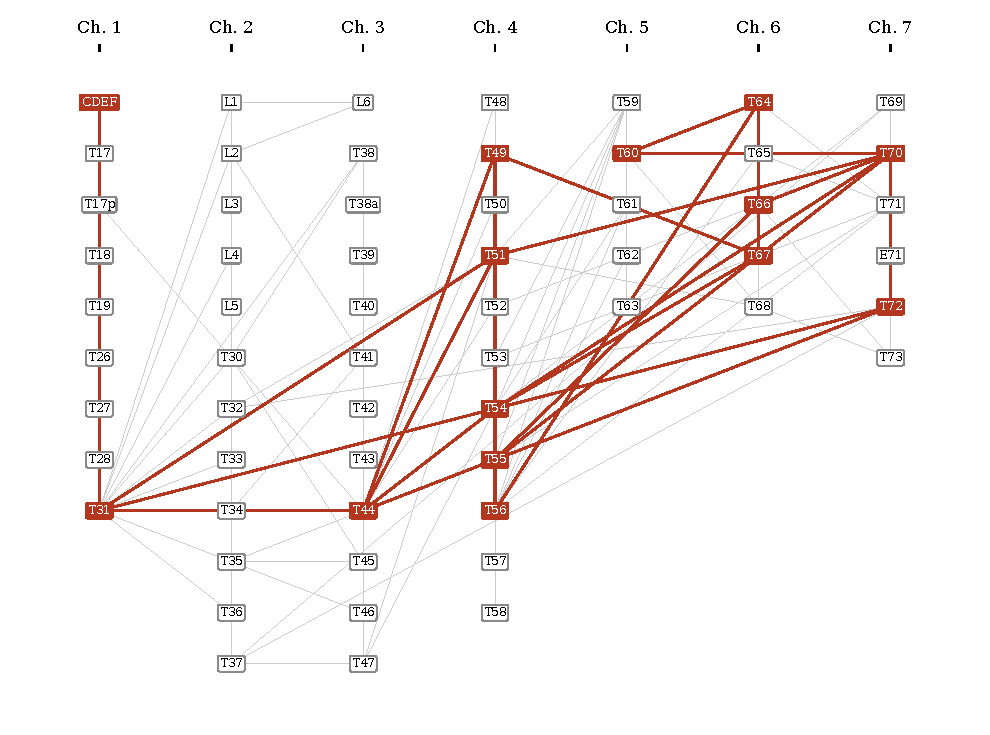
\includegraphics[width=0.98\linewidth]{figs/fig_dag.pdf}
\caption{The proof-dependency graph of the 60 theorem-type records of this volume (nodes arranged in the seven manuscript chapters; \(60\) nodes, \(139\) edges within the volume). Red edges: the main line of the argument. Records of earlier chapters appear as dependencies of later ones, never the reverse.}\label{fig:dag}
\end{figure}

\section*{Table of direct dependencies}

Direct proof dependencies of the records of this volume, as listed in the registry (records of Volume~I appear as dependencies where used).

\footnotesize
\begin{longtable}{@{}p{14mm}p{108mm}@{}}
\toprule Record & Depends on (registry dependency list)\\\midrule\endfirsthead
\toprule Record & Depends on (registry dependency list)\\\midrule\endhead
\texttt{CDEF} & \texttt{T8} \\
\texttt{T17p} & \texttt{T8} \\
\texttt{T17} & \texttt{CDEF, T17p} \\
\texttt{T18} & \texttt{T17, T1} \\
\texttt{T19} & \texttt{T18, T17} \\
\texttt{T26} & \texttt{T18} \\
\texttt{T27} & \texttt{T17, T18} \\
\texttt{T28} & \texttt{T6, CDEF} \\
\texttt{T30} & \texttt{T22, T17p} \\
\texttt{T31} & \texttt{T30, CDEF} \\
\texttt{T32} & \texttt{T30, T31, T22} \\
\texttt{T33} & \texttt{T31, T32, T30} \\
\texttt{T34} & \texttt{T30} \\
\texttt{L1} & \texttt{T30, T31} \\
\texttt{L2} & \texttt{T30, T31, L1} \\
\texttt{L3} & \texttt{T32} \\
\texttt{L4} & \texttt{L3, T31} \\
\texttt{L5} & \texttt{T33, L4} \\
\texttt{L6} & \texttt{L1, L2} \\
\texttt{T35} & \texttt{T1, T31} \\
\texttt{T36} & \texttt{T35, T31} \\
\texttt{T37} & \texttt{L1} \\
\texttt{T38} & \texttt{T31, T30, T22} \\
\texttt{T38a} & \texttt{T38} \\
\texttt{T39} & \texttt{T38, T38a} \\
\texttt{T40} & \texttt{T38} \\
\texttt{T41} & \texttt{T34, L2, T38} \\
\texttt{T42} & \texttt{T38} \\
\texttt{T43} & \texttt{T38, T46} \\
\texttt{T44} & \texttt{T30, T31, T35} \\
\texttt{T45} & \texttt{T44, T30, T35} \\
\texttt{T46} & \texttt{T38, T44, T31} \\
\texttt{T47} & \texttt{T44, T37} \\
\texttt{T48} & \texttt{T44} \\
\texttt{T49} & \texttt{T44} \\
\texttt{T50} & \texttt{T49, T44} \\
\texttt{T51} & \texttt{T49, T47, T44, T32, T31} \\
\texttt{T52} & \texttt{T49, T44} \\
\texttt{T53} & \texttt{T49} \\
\texttt{T54} & \texttt{T53, T44, T47} \\
\texttt{T55} & \texttt{T54, T53, T51} \\
\texttt{T56} & \texttt{T54, T55, T53} \\
\texttt{T57} & \texttt{T49, T54, T53, T56} \\
\texttt{T58} & \texttt{T50, T57, T54, T48} \\
\texttt{T59} & \texttt{T53, T54, T55, T56, T51} \\
\texttt{T60} & \texttt{T59} \\
\texttt{T61} & \texttt{T60, T56, T54} \\
\texttt{T62} & \texttt{T56} \\
\texttt{T63} & \texttt{T60} \\
\texttt{T67} & \texttt{T53, T54, T49} \\
\texttt{T64} & \texttt{T56, T60} \\
\texttt{T65} & \texttt{T56} \\
\texttt{T66} & \texttt{T64, T65, T67, T52, T55} \\
\texttt{T68} & \texttt{T66, T51, T60} \\
\texttt{T69} & \texttt{T54, T44, T37} \\
\texttt{T70} & \texttt{T51, T52, T54, T55, T60, T66, T67} \\
\texttt{T71} & \texttt{T55, T64, T67, T56, T65} \\
\texttt{T72} & \texttt{T31, T44, T37, T69, T70, T32} \\
\texttt{T73} & \texttt{T68, T66, T69, T70, T71, T72} \\
\texttt{O12.1} & \texttt{T70, T71, T72} \\
\texttt{O12.2} & \texttt{T66, T73} \\
\texttt{O12.3} & \texttt{T71, T67} \\
\texttt{O12.4} & \texttt{T57, T64, T65} \\
\texttt{O12.5} & \texttt{T57} \\
\texttt{O12.6} & \texttt{T51, T57} \\
\texttt{O10.3} & \texttt{T56, T62, T52} \\
\texttt{O10.4} & \texttt{T60} \\
\texttt{E71} & \texttt{T71} \\
\bottomrule
\end{longtable}
\normalsize

